\documentclass[utf8]{frontiers_suppmat}
\usepackage{url,hyperref,microtype,booktabs,longtable}
\usepackage[singlespacing]{setspace}
\hypersetup{hidelinks}
\setlength{\headheight}{20pt}
\setlength{\headsep}{15pt}
\newcommand{\SupplementFeasRows}{%
6 & 31.25 & 62.42 & 89.96 & 88.00 & 100.00 \\
8 & 21.88 & 40.57 & 76.26 & 73.00 & 100.00 \\
9 & 10.55 & 31.68 & 63.46 & 63.00 & 100.00 \\
10 & 11.72 & 41.37 & 77.88 & 70.50 & 100.00 \\
12 & 3.96 & 32.51 & 31.18 & 29.50 & 100.00 \\
15 & 1.10 & 34.85 & 68.70 & 65.00 & 100.00 \\
}

\newcommand{\SupplementHitRows}{%
6 & 95.71 & 84.89 & 96.04 & 100.00 \\
8 & 54.29 & 93.63 & 99.21 & 97.28 \\
9 & 32.36 & 10.42 & 16.94 & 97.62 \\
10 & 17.75 & 80.45 & 94.02 & 81.24 \\
12 & 4.77 & 28.23 & 31.88 & 71.02 \\
15 & 0.61 & 25.02 & 39.01 & 42.67 \\
}

\newcommand{\PanelRows}{
1 & 0 & 64.00 & 2.682 & 1.265 & 0.617\\
1 & 1 & 61.68 & 2.230 & 1.265 & 0.617\\
1 & 2 & 64.75 & 2.752 & 1.265 & 0.617\\
2 & 0 & 63.42 & 3.365 & 1.485 & 0.617\\
2 & 1 & 62.65 & 3.319 & 1.485 & 0.617\\
2 & 2 & 63.91 & 3.427 & 1.485 & 0.617\\
3 & 0 & 64.89 & 3.279 & 1.436 & 0.617\\
3 & 1 & 64.31 & 3.248 & 1.436 & 0.617\\
3 & 2 & 64.05 & 3.219 & 1.436 & 0.617\\
4 & 0 & 66.51 & 2.894 & 1.295 & 0.617\\
4 & 1 & 65.66 & 2.809 & 1.295 & 0.617\\
4 & 2 & 66.05 & 2.865 & 1.295 & 0.617\\
}

\newcommand{\QualityRows}{
6 & 33.5 & 0.0 & 0.0 & 21\\
8 & 38.3 & 0.0 & 0.0 & 37\\
9 & 33.5 & 22.1 & 0.0 & 33\\
10 & 38.3 & 30.3 & 0.0 & 53\\
12 & 34.5 & 39.5 & 0.0 & 57\\
15 & 39.7 & 18.8 & 0.0 & 81\\
}

\newcommand{\RecoveredQualityRows}{%
6 & 2 & 07-03 03:33 & 442 & 35.2 & 0.0 & 21\\
6 & 2 & 07-03 05:16 & 176 & 33.5 & 0.0 & 21\\
6 & 2 & 07-11 07:10 & 171 & 35.5 & 0.0 & 21\\
8 & 2 & 07-03 05:25 & 146 & 38.3 & 0.0 & 37\\
8 & 2 & 07-11 07:12 & 144 & 36.2 & 0.0 & 37\\
9 & 3 & 07-03 05:33 & 126 & 33.5 & 22.1 & 33\\
10 & 2 & 07-03 05:41 & 141 & 38.3 & 30.3 & 53\\
10 & 2 & 07-11 07:19 & 139 & 40.4 & 0.0 & 53\\
12 & 2 & 07-11 07:25 & 145 & 53.1 & 0.0 & 69\\
12 & 3 & 07-03 05:51 & 59 & 34.5 & 39.5 & 57\\
14 & 2 & 07-11 07:38 & 124 & 50.0 & 0.0 & 85\\
15 & 3 & 07-03 06:03 & 130 & 39.7 & 18.8 & 81\\
15 & 3 & 07-11 07:48 & 109 & 40.1 & 16.2 & 81\\
18 & 3 & 07-11 06:06 & 84 & 48.9 & 12.5 & 105\\
18 & 3 & 07-11 07:55 & 99 & 47.1 & 0.0 & 105\\
18 & 3 & 07-12 13:37 & 92 & 50.0 & 0.0 & 105\\
20 & 5 & 07-11 08:09 & 40 & 37.7 & 27.9 & 97\\
20 & 5 & 07-12 13:47 & 54 & 37.7 & 27.9 & 97\\
21 & 3 & 07-11 06:09 & 88 & 49.0 & 0.0 & 129\\
21 & 3 & 07-11 08:02 & 81 & 47.4 & 26.3 & 129\\
21 & 3 & 07-12 13:40 & 70 & 47.8 & 26.7 & 129\\
25 & 5 & 07-11 08:17 & 26 & 39.3 & 9.1 & 137\\
25 & 5 & 07-12 13:54 & 30 & 38.6 & 20.5 & 137\\
30 & 5 & 07-11 08:23 & 13 & 43.1 & 35.0 & 177\\
35 & 5 & 07-11 08:33 & 7 & 47.5 & 40.4 & 200\\
}

\newcommand{\LargerControlRows}{%
18 & 675 & Ideal QAOA & 73.16 & 0.1666 & 51.0 \\
18 & 675 & Initial product & 37.37 & 0.0985 & 51.2 \\
18 & 675 & Uniform feasible & 100.00 & 0.1481 & 41.8 \\
20 & 650 & Ideal QAOA & 25.52 & 0.0239 & 39.0 \\
20 & 650 & Initial product & 27.80 & 0.0212 & 38.1 \\
20 & 650 & Uniform feasible & 100.00 & 0.1538 & 31.8 \\
21 & 1134 & Ideal QAOA & 73.44 & 0.1111 & 49.3 \\
21 & 1134 & Initial product & 39.11 & 0.0670 & 49.5 \\
21 & 1134 & Uniform feasible & 100.00 & 0.0882 & 40.3 \\
25 & 1500 & Ideal QAOA & 29.53 & 0.0242 & 42.4 \\
25 & 1500 & Initial product & 30.72 & 0.0222 & 42.0 \\
25 & 1500 & Uniform feasible & 100.00 & 0.0667 & 33.4 \\
30 & 2875 & Ideal QAOA & 33.39 & 0.0174 & 52.1 \\
30 & 2875 & Initial product & 33.64 & 0.0172 & 52.0 \\
30 & 2875 & Uniform feasible & 100.00 & 0.0348 & 43.2 \\
35 & 4900 & Ideal QAOA & 35.85 & 0.0120 & 50.3 \\
35 & 4900 & Initial product & 35.75 & 0.0122 & 50.3 \\
35 & 4900 & Uniform feasible & 100.00 & 0.0204 & 41.7 \\
}

\newcommand{\LargerHardwareRows}{%
18 & 07-11 06:06 & 42.0 & 0.0 & 48.9 \\
18 & 07-11 07:55 & 49.5 & 0.5 & 47.1 \\
18 & 07-12 13:37 & 46.0 & 0.5 & 50.0 \\
20 & 07-11 08:09 & 20.0 & 0.0 & 37.7 \\
20 & 07-12 13:47 & 27.0 & 0.0 & 37.7 \\
21 & 07-11 06:09 & 44.0 & 0.5 & 49.0 \\
21 & 07-11 08:02 & 40.5 & 0.0 & 47.4 \\
21 & 07-12 13:40 & 35.0 & 0.0 & 47.8 \\
25 & 07-11 08:17 & 13.0 & 0.0 & 39.3 \\
25 & 07-12 13:54 & 15.0 & 0.0 & 38.6 \\
30 & 07-11 08:23 & 6.5 & 0.0 & 43.1 \\
35 & 07-11 08:33 & 3.5 & 0.0 & 47.5 \\
}

\begin{document}
\onecolumn
\firstpage{1}
\title[Supplementary Material]{{\helveticaitalic{Supplementary Material}}}
{\setlength{\parindent}{0pt}\maketitle}

\section{Hardware dataset}
We analyze 25 completed IonQ Forte-1 tasks, counting one duplicate 10-qubit download once. Twenty-four tasks have 200 shots and one 6-qubit task has 500 shots, totaling 5,300. Each record contains the measured-qubit order, submitted OpenQASM, output probabilities and task metadata. Every circuit matches an archived instance definition.

The analysis is retrospective and was not preregistered. We use the drug-response data to construct the optimization instances and the hardware records to assess circuit outputs. Figures are generated from the analyzed records.

Main Table~1 and Figures~1A and 2 report the original six-task series and its independently checked noiseless calculations. Figure~1B compares larger circuits with their noiseless predictions. Main Table~2 reports the other 19 tasks. Together, the records contain 18 distinct circuits and 14 optimization instances, including the 30- and 35-qubit executions.

The reproducibility package contains the original JSON files, four archived runner scripts, instance definitions and SHA-256 hashes. The task UUIDs are listed below.

\section{Circuit identity and independent calculations}
We extract literal instance arrays from the four archived runners using Python's abstract syntax tree, without importing or executing the submission code. We reconstruct the initial $R_y$ rotations, cost $R_z$ rotations and CNOT pairs, and final $R_y(-\theta)$, $R_z(2\beta)$, $R_y(\theta)$ mixers. We check each operation, wire and angle against the submitted OpenQASM, with an absolute angle tolerance of $10^{-10}$. Native compiled programs are unavailable, so the records cannot establish native-gate counts or noise parameters.

A NumPy simulator applies the submitted gate sequence. A second calculation applies the diagonal Ising phase and tensor-product mixers. For the original six instances, their full probability vectors agree within $10^{-10}$ maximum absolute error. PennyLane \texttt{default.qubit} checks the same gate list within $10^{-12}$ absolute tolerance. Bell-state and single-wire rotation tests check bit order: the first outcome character represents wire zero.

We construct the feasible sets independently by decoding binary states and enumerating compound assignments. The reconstructed decoding, feasibility and scoring functions match the originals on all 38,720 binary states across the six reference instances; scores are compared only for feasible states. Enumeration checks for tied optima and finds one optimum per instance. For the expanded models, we enumerate compound subsets and doses, check them against Cartesian assignment enumeration, and compare bit-level and assignment-level scores. The 35-qubit model has 4,900 feasible assignments. We also decode every observed output independently. Larger-circuit noiseless calculations are described below. Coefficients retain their archived precision.

\section{Classical sampling and uncertainty}
The 10-qubit prior feasibility is 41.36\% when truncated to two decimal places; Table~S1 rounds this value to 41.37\%.

To sample uniformly from the feasible set, choose $m=2$ or $3$ with probability proportional to $\binom{n}{m}D^m$, choose an $m$-compound subset uniformly, and draw one of $D$ doses independently for each selected compound. Every compound has a distinct mechanism class, so each feasible assignment has equal probability. Sampling uses only the constraints.

For warm-start-only sampling, draw each bit independently with probability $\sin^2(\theta_v/2)$. We calculate feasible and optimum probabilities by summing over the corresponding states. Ideal-QAOA probabilities are calculated in the same way.

For $k$ successes in $N$ shots, the reported 95\% Wilson interval is
\begin{equation}
 \frac{\hat p+z^2/(2N)\ \pm\ z\sqrt{\hat p(1-\hat p)/N+z^2/(4N^2)}}{1+z^2/N},
 \quad \hat p=k/N,\quad z=1.9599639845.
\end{equation}
The pointwise intervals assume independent shots within each run. They exclude unrecorded calibration changes, provider processing and variation between runs. We make no multiple-comparison claims.

The main fixed-budget metric, $1-(1-P_\star)^{200}$, gives the probability of finding at least one optimum in 200 independent draws with replacement from an analytically known distribution. Hardware columns report observed batches separately. Tables~S4--S5 summarize scores conditional on feasibility. The code also records the expected normalized best-of-200 score for the analytic controls.

\section{Exact control probabilities}
\begin{table}[h!]
\caption{Feasible probability (percent) for the analytic controls and archived hardware outputs. Uniform feasible sampling returns a valid assignment in 100\% of draws.}
\centering\small
\begin{tabular}{rrrrrr}
\toprule
Qubits & Uniform bits & Initial product & Ideal QAOA & Hardware & Uniform feasible\\
\midrule
\SupplementFeasRows
\bottomrule
\end{tabular}
\end{table}

\begin{table}[h!]
\caption{Probability of finding at least one optimum in 200 independent draws (percent) from the analytic controls. Hardware batches are reported separately.}
\centering\small
\begin{tabular}{rrrrr}
\toprule
Qubits & Uniform bits & Initial product & Ideal QAOA & Uniform feasible\\
\midrule
\SupplementHitRows
\bottomrule
\end{tabular}
\end{table}

\section{Model coefficients and circuit parameters}
The file \texttt{CAMA1c7\_D3\_meta.json} and coefficient arrays define the seven-compound CAMA-1 model. The source builder retains QA-passing AstraZeneca--Sanger DREAM observations, averages pairwise synergy values and takes the median monotherapy Hill parameters. The single-agent term is $h_{id}=[100-v_i(c_d)]/100$, with
\begin{equation}
v_i(c)=E_{\infty,i}+\frac{100-E_{\infty,i}}{1+(c/IC_{50,i})^{H_i}}.
\end{equation}
The pair term is $J_{id,je}=s_{ij}c_dc_e/100$, where $s_{ij}$ is the archived synergy coefficient. The dose proxy $t_{id}=w_i c_d$ uses an illustrative mechanism-class weight. We retain the coefficients without refitting. Source arrays, metadata, builder code and hashes are included in the package.

For the new panels, define $l_v=h_v-0.6t_v$, $S=\sum_v x_v$ and $S_i$ as the number of active dose bits for compound $i$. The minimized cost, up to a constant, is
\begin{equation}
C(x)=-f(x)+P(S-2)(S-3)+P\sum_i S_i(S_i-1),
\end{equation}
where $P=3[\max_v|l_v|+\max_v\sum_w|J_{vw}|+10^{-6}]$ and $J$ is the symmetric score-interaction matrix. The second penalty adds $2P$ for each pair of active bits in a compound block. Distinct class labels make a mechanism-class penalty unnecessary. We check the reconstructed Ising energy against this polynomial for every binary state, allowing for the constant shift.

Initialization uses standardized linear scores $g_v=(l_v-\bar l)/\mathrm{sd}(l)$, or the unstandardized scores when the standard deviation is below $10^{-9}$. We set $a_v=[1+\exp(-g_v/0.5)]^{-1}$, $c_v=\mathrm{clip}[2.5a_v/\sum_w a_w,0.001,0.999]$ and $\theta_v=2\arcsin\sqrt{c_v}$. Each seed draws $\gamma,\beta$ independently from $N(0,0.1^2)$ and performs 60 Adam updates of the expected penalized cost. The learning rate is 0.1, moment coefficients are 0.9 and 0.99, and stabilizer is $10^{-8}$, matching the source optimizer. We retain every final iterate, initialization and circuit. Gradient and cost trajectories are archived for the original four-panel experiment; expanded runs store initializations and final results. All new panels use this training rule. Historical hardware training trajectories are unavailable.

\section{Panel and initialization sensitivity}
Before optimization, we use NumPy seed 20260905 to draw four panels without replacement from the lexicographically ordered 35 four-compound subsets of the archived seven-compound order:
\begin{itemize}
\item Panel 1: FASN, MAP2K\_1, PIK3CB\_PIK3CD, SLC16A4.
\item Panel 2: AKT\_1, FASN, MTOR\_1, SLC16A4.
\item Panel 3: FASN, MAP2K\_1, MTOR\_1, PIK3CB\_PIK3CD.
\item Panel 4: BCL2\_BCL2L1, FASN, MTOR\_1, SLC16A4.
\end{itemize}
Each panel has 12 qubits, 162 feasible assignments and one optimum. The package records the design and source-file hashes. Table~S3 includes all three initialization seeds per panel; Table~S11 reports the expanded CAMA-1 and second-cell-line results.

\begin{table}[h!]
\caption{Noiseless results for four panels and three seeds per panel. Valid: feasible probability. Other probability columns report per-shot optimum recovery. All probabilities are percentages; uniform feasible sampling gives $100/162$. Greedy search finds the four panel optima in 36, 50, 36 and 36 evaluations, respectively.}
\centering\small
\begin{tabular}{rrrrrr}
\toprule
Panel & Seed & Valid & Ideal optimum & Prior optimum & Feasible optimum\\
\midrule
\PanelRows
\bottomrule
\end{tabular}
\end{table}

The four panel optimum scores are 0.327939, 0.732473, 0.532951 and 0.143720, respectively. Simulations use NumPy on Pawsey Setonix ARM CPUs. We check the statevector gradients and Adam updates against PennyLane.

\section{Solution quality and repeated executions}
\begin{table}[h!]
\caption{Feasible solution quality and greedy search for the original six tasks. Mean quality is $100\,\mathbb{E}[u\mid\mathcal F]$; best gap is $100(1-\max u)$ over valid shots. Greedy gaps use the same score range. The search cap is 200 unique objective evaluations, including partial construction. Counts exclude quantum training and execution costs.}
\centering\small
\begin{tabular}{rrrrr}
\toprule
$q$ & HW mean quality (\%) & HW best gap (\%) & Greedy gap (\%) & Eval.\\
\midrule
\QualityRows
\bottomrule
\end{tabular}
\end{table}

\begin{table}[h!]
\caption{Feasible solution quality for all 25 tasks. Dates and times are UTC in 2026. Valid: feasible-shot count. Mean and best gap use the percentage normalization in Table~S4. Greedy: total unique score evaluations, including partial construction. Every search reaches its exact optimum; repeated problems share the deterministic search result.}
\centering\small
\begin{tabular}{rrlrrrr}
\toprule
$q$ & $D$ & UTC date/time & Valid & Mean & Best gap & Greedy\\
\midrule
\RecoveredQualityRows
\bottomrule
\end{tabular}
\end{table}

Identical circuits have two executions at 6 qubits, three at 18, two at 20, three at 21 and two at 25. Each task has its own identifier, histogram, shot denominator and Wilson interval. The limited repeats and missing calibration records prevent estimates of long-term drift or equivalence between executions. Additional programs at 6, 8, 10 and 15 qubits use different angles from the original series; the two 12-qubit programs encode different instances. We analyze those tasks separately. The runner records transferred parameters for the 25-, 30- and 35-qubit circuits.

\section{Hardware score distributions}
We normalize valid hardware scores by the full feasible score range: $u=(f-f_{\min})/(f_\star-f_{\min})$. Figure~S1 shows the empirical cumulative distribution among valid outputs, with each panel's valid-shot denominator. Means and best scores describe the observed batch.

\begin{figure}[h!]
\centering
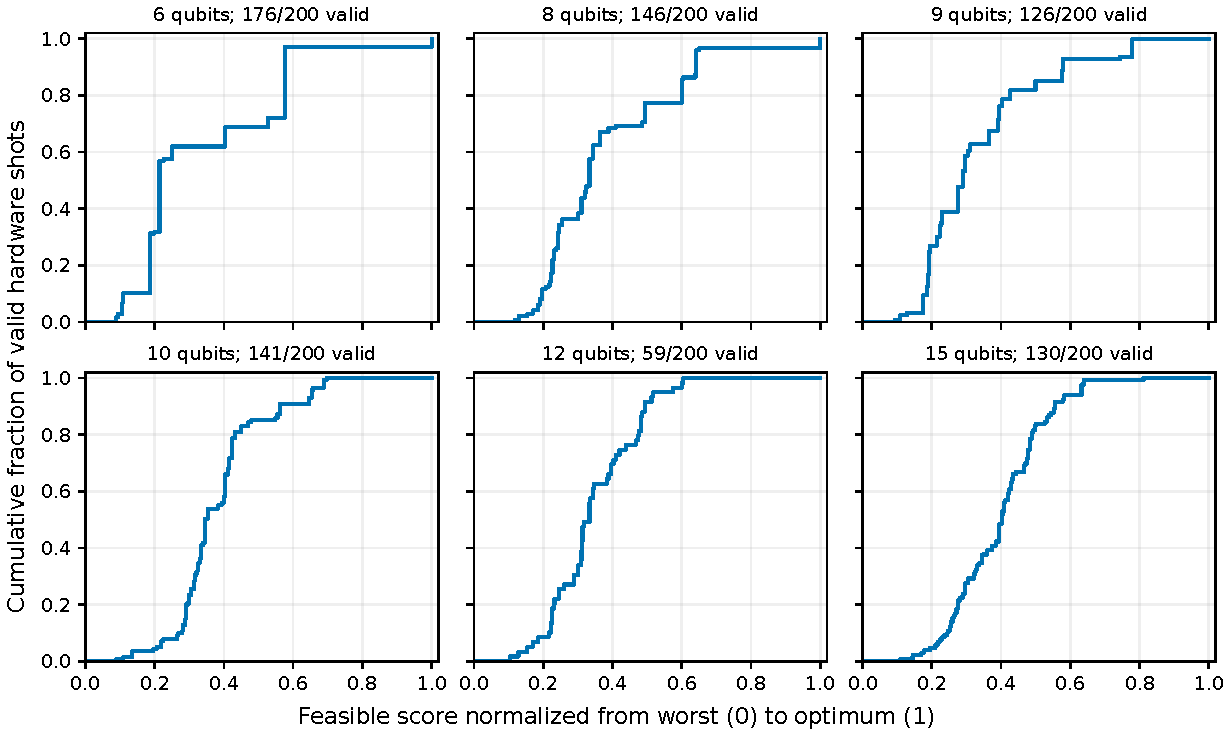
\includegraphics[width=\textwidth]{figures/figureS1.pdf}
\caption{Feasible-score distributions for the original six hardware batches in main Table~1. The horizontal axis ranges from the worst feasible score (zero) to the optimum (one). The vertical axis gives the fraction of valid shots at or below each score. Invalid outputs are counted in the main feasibility analysis.}
\end{figure}

\begin{figure}[h!]
\centering
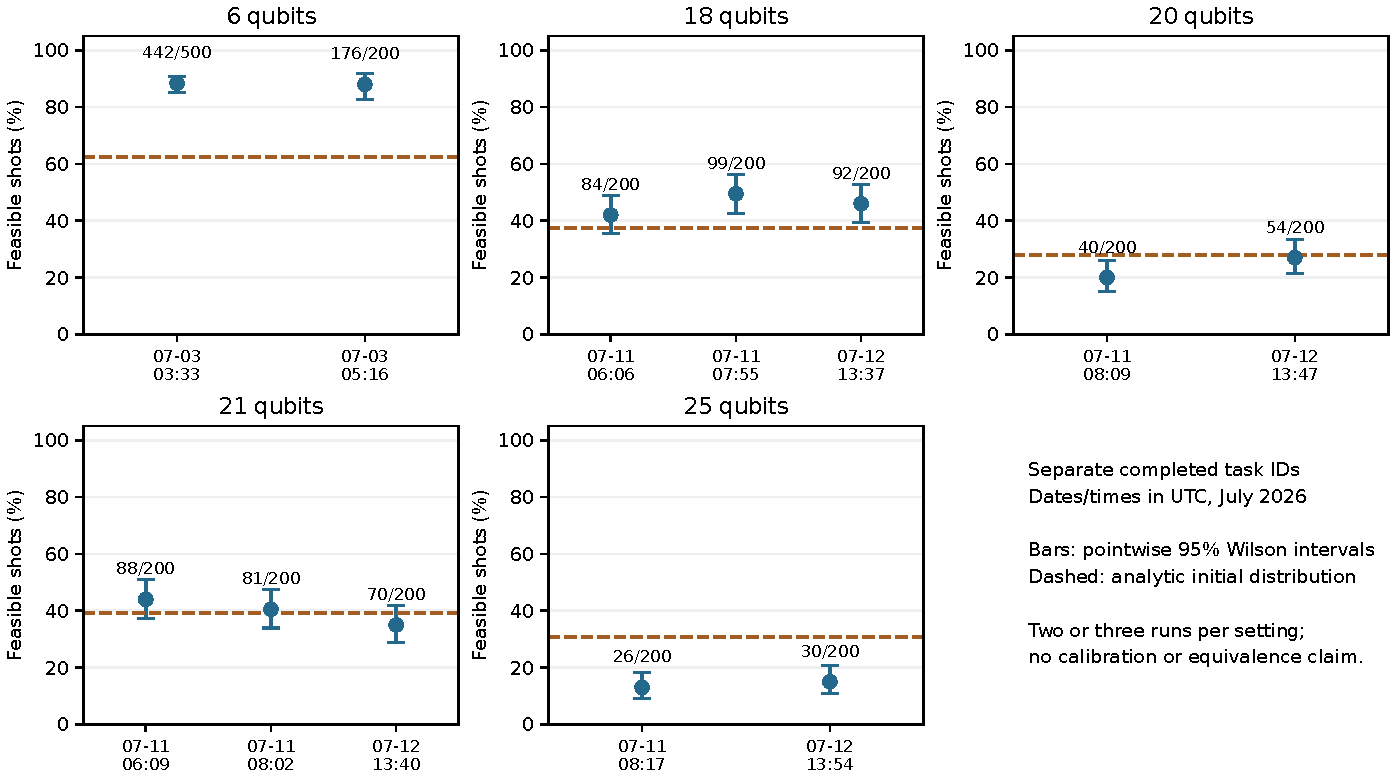
\includegraphics[width=\textwidth]{figures/figureS2.pdf}
\caption{Repeated executions of identical circuits. Each marker represents one task; labels give valid/total shots. Error bars are pointwise 95\% Wilson intervals. Dashed lines show analytic initial-product feasibility. Dates and times are UTC.}
\end{figure}

\clearpage
\section{Larger-circuit noiseless references}
We calculate statevectors for the archived 18-, 20-, 21- and 25-qubit circuits using their original angles and coefficients. One circuit at each width corresponds to three, two, three and two hardware executions, respectively; each group shares one reference distribution. We form initial amplitudes and diagonal Ising phases in chunks of $2^{18}$ integer indices. For index $j$, the bit on wire $v$ is $(j\mathbin{\mathrm{div}}2^{q-1-v})\bmod 2$; bit parity gives pairwise $Z$ eigenvalues. Local mixers update disjoint amplitude pairs in place with bounded temporary arrays. Working memory is $O(2^q+C)$ for chunk size $C$, avoiding a $2^q\times q$ bit matrix. The 25-qubit complex128 statevector occupies 512 MiB. Full-statevector storage still grows exponentially with circuit width.

We decode feasible assignments into a bit matrix and sum their probabilities for feasibility. Summing over all tied optima gives optimum probability; probability-weighted scores give conditional mean quality. The four feasible sets contain 675, 650, 1,134 and 1,500 assignments; the added sets contain 2,875 and 4,900. Each has one optimum. Initial-product and uniform-feasible controls use the same checked assignments. Table~S6 reports the controls and Table~S7 the hardware batches. Machine-readable results include unnormalized mean scores, full-precision probabilities, task UUIDs and source hashes.

The chunked implementation reproduces all six original probability vectors within $10^{-12}$. At 18 qubits, independent simulation of the submitted gate sequence agrees within $10^{-10}$. All four final state norms differ from one by less than $10^{-10}$.

The calculations use Python 3.11.7 and NumPy 1.24.4 on Pawsey Setonix ARM CPUs. The 30- and 35-qubit calculations, with 2,875 and 4,900 feasible assignments, use Numba 0.60.0 and complex64 amplitudes. Their statevectors occupy 8 GiB and 256 GiB, respectively. We allocate four GPU shares for host memory and calculate on 72 CPU threads without GPU kernels.

We initialize amplitudes and phases in Gray-code order within blocks of $2^{16}$ states. Each transition changes one bit, so energy updates use only that bit's incident interactions. We recompute the starting amplitude and energy at each block boundary, then apply local mixers to disjoint amplitude pairs in parallel. The result archive stores feasible-state probabilities for rescoring and omits full statevectors.

At 25 qubits, the maximum complex64 amplitude error relative to complex128 is $4.14\times10^{-8}$; total feasible probability differs by $2.29\times10^{-10}$. The maximum relative error among feasible probabilities is $7.77\times10^{-7}$. Both precisions pass independent comparisons on all six original circuits. The 30- and 35-qubit state norms differ from one by less than $4\times10^{-8}$. Calculations take 8.90 and 270.46 seconds, respectively, excluding queueing and setup. These timings measure simulation only and exclude quantum hardware training and execution.

\begin{table}[h!]
\caption{Noiseless and classical controls for six circuits. Probabilities and normalized quality are rounded percentages. $|\mathcal F|$: feasible assignments; $P_{\mathcal F}$: feasible probability; $P_\star$: per-draw optimum probability; mean $u$: quality conditional on feasibility. Identical hardware repetitions share one ideal reference.}
\centering\small
\begin{tabular}{rrlrrr}
\toprule
$q$ & $|\mathcal F|$ & Distribution & $P_{\mathcal F}$ & $P_\star$ & Mean $u$\\
\midrule
\LargerControlRows
\bottomrule
\end{tabular}
\end{table}

\begin{table}[h!]
\caption{Hardware executions corresponding to Table~S6. Each batch has 200 shots; values are percentages. Dates and times are UTC in 2026. $P_\star$ is the observed optimum fraction. Main Table~2 and Figure~1B give pointwise feasibility intervals; Table~S5 gives best-sample gaps.}
\centering\small
\begin{tabular}{rlrrr}
\toprule
$q$ & UTC date/time & Feasible & Optimum & Mean $u$\\
\midrule
\LargerHardwareRows
\bottomrule
\end{tabular}
\end{table}

\clearpage
\clearpage
\section{Additional classical search and panel definitions}
We use simulated annealing (SA) with the same feasible dose-change, addition, deletion and compound-swap neighborhood as greedy local search. We draw the initial assignment uniformly from the feasible space by rejection sampling complete compound assignments. At each step we propose a uniformly chosen neighbor and accept an improving move, or accept a worse move with probability $\exp(\Delta f/T)$. We use 100 seeds, numbered 0 through 99, for each model and weight.

We set the initial temperature to the maximum absolute linear or pair coefficient, with a lower bound of $10^{-6}$. Over 2,000 proposals we cool geometrically to one thousandth of that temperature. We stop after 200 unique objective evaluations or 2,000 proposals, whichever comes first. Cached evaluations do not count again. The initial state's evaluation counts toward the cap. For small feasible sets the proposal limit prevents an endless attempt to obtain 200 distinct evaluations. We record the best score evaluated, and compare its trace with the enumerated optimum only after the run. Median first-hit evaluations condition on successful seeds; the success fraction reports failures separately.

Exhaustive enumeration is the exact solver: it evaluates each feasible assignment once. It supplies no search information to SA or greedy. Table~S8 reports all hardware models and the expanded panels at the archived weight. OR-Tools is not installed in the execution environment, so CP-SAT is not included.

\begingroup
\small
\setlength{\tabcolsep}{4pt}
\begin{longtable}{lrrrrrr}
\caption{Classical search at $\lambda=0.6$. H01--H14 are hardware models, C01--C35 are all CAMA-1 panels, and V1--V4 are 647-V panels. Exact: enumeration evaluations, equal to $|\mathcal F|$. Greedy: total unique evaluations, including partial construction states, and optimum recovery. SA: percentage of 100 seeds reaching the optimum and median evaluations to first hit among successful seeds.}\\
\toprule
Model & $q$ & Exact & Greedy eval. & Hit & SA (\%) & First hit\\
\midrule
\endfirsthead
\toprule
Model & $q$ & Exact & Greedy eval. & Hit & SA (\%) & First hit\\
\midrule
\endhead
H01 & 6 & 20 & 21 & yes & 100 & 11 \\
H02 & 8 & 56 & 37 & yes & 100 & 20.5 \\
H03 & 9 & 54 & 33 & yes & 100 & 22.5 \\
H04 & 10 & 120 & 53 & yes & 100 & 36 \\
H05 & 12 & 162 & 57 & yes & 100 & 54 \\
H06 & 15 & 360 & 81 & yes & 98 & 87.5 \\
H07 & 18 & 675 & 105 & yes & 68 & 112.5 \\
H08 & 21 & 1134 & 129 & yes & 65 & 115 \\
H09 & 20 & 650 & 97 & yes & 65 & 115 \\
H10 & 25 & 1500 & 137 & yes & 33 & 127 \\
H11 & 12 & 220 & 69 & yes & 100 & 57 \\
H12 & 14 & 364 & 85 & yes & 95 & 77 \\
H13 & 30 & 2875 & 177 & yes & 22 & 97.5 \\
H14 & 35 & 4900 & 200 & yes & 15 & 144 \\
C01 & 12 & 162 & 36 & yes & 100 & 56 \\
C02 & 12 & 162 & 50 & yes & 100 & 56.5 \\
C03 & 12 & 162 & 50 & yes & 100 & 58 \\
C04 & 12 & 162 & 36 & yes & 100 & 61.5 \\
C05 & 12 & 162 & 50 & yes & 100 & 56 \\
C06 & 12 & 162 & 50 & yes & 100 & 49.5 \\
C07 & 12 & 162 & 36 & yes & 100 & 58.5 \\
C08 & 12 & 162 & 57 & yes & 100 & 47 \\
C09 & 12 & 162 & 50 & yes & 100 & 43.5 \\
C10 & 12 & 162 & 59 & yes & 100 & 66 \\
C11 & 12 & 162 & 50 & yes & 100 & 55.5 \\
C12 & 12 & 162 & 50 & yes & 100 & 58 \\
C13 & 12 & 162 & 36 & yes & 100 & 65 \\
C14 & 12 & 162 & 57 & yes & 100 & 50.5 \\
C15 & 12 & 162 & 50 & yes & 100 & 48.5 \\
C16 & 12 & 162 & 59 & yes & 100 & 62 \\
C17 & 12 & 162 & 57 & yes & 100 & 45 \\
C18 & 12 & 162 & 50 & yes & 100 & 43.5 \\
C19 & 12 & 162 & 59 & yes & 100 & 69.5 \\
C20 & 12 & 162 & 57 & yes & 100 & 54 \\
C21 & 12 & 162 & 36 & yes & 100 & 65 \\
C22 & 12 & 162 & 36 & yes & 100 & 53 \\
C23 & 12 & 162 & 36 & yes & 100 & 63.5 \\
C24 & 12 & 162 & 36 & yes & 100 & 45.5 \\
C25 & 12 & 162 & 36 & yes & 100 & 69.5 \\
C26 & 12 & 162 & 36 & yes & 100 & 60.5 \\
C27 & 12 & 162 & 36 & yes & 100 & 65.5 \\
C28 & 12 & 162 & 36 & yes & 100 & 59 \\
C29 & 12 & 162 & 36 & yes & 100 & 50.5 \\
C30 & 12 & 162 & 36 & yes & 100 & 38 \\
C31 & 12 & 162 & 36 & yes & 100 & 49 \\
C32 & 12 & 162 & 36 & yes & 100 & 53.5 \\
C33 & 12 & 162 & 36 & yes & 100 & 60 \\
C34 & 12 & 162 & 36 & yes & 100 & 52 \\
C35 & 12 & 162 & 36 & yes & 100 & 54 \\
V1 & 12 & 162 & 46 & yes & 100 & 58 \\
V2 & 12 & 162 & 46 & yes & 100 & 48.5 \\
V3 & 12 & 162 & 55 & yes & 100 & 58.5 \\
V4 & 12 & 162 & 50 & no & 100 & 84 \\
\bottomrule
\end{longtable}
\endgroup

Hardware model labels follow the original six instances first, then the additional distinct models. Their compound counts, dose counts and feasible-set sizes identify the encoding; Table~S9 additionally identifies every distinct circuit. Panel membership is given with Table~S11.

\clearpage
\section{Score-weight sensitivity}
We retain $\lambda=0.6$ as the archived model value and rescore each feasible assignment at $\lambda\in\{0.3,0.45,0.6,0.75,0.9\}$. All archived circuit coefficients, initialization angles, variational angles and hardware histograms remain fixed. Only the score and the set of globally optimal feasible assignments change. We sum each fixed distribution over that new optimum set, including ties. For the original four 12-qubit panels we instead rebuild the penalty cost and product prior at each weight and retrain all three seeds with 60 Adam steps and learning rate 0.1. Table~S9 distinguishes those retrained panels (P1--P4) from the fixed circuits (Q01--Q18).

Each entry below is a per-draw optimum probability, in percent. Hardware values are observed fractions, with repeated tasks separated by slashes in chronological order. A dash indicates an unavailable noiseless reference. Greedy reports whether it reaches the re-enumerated optimum; SA gives the percentage of successful seeds. For retrained panels the ideal values follow seed order 0, 1 and 2. The machine-readable results include exact optimum scores, all tied optimum bitstrings, individual hardware task identifiers and every SA seed.

\begingroup
\small
\setlength{\tabcolsep}{4pt}
\begin{longtable}{rrrrlrrr}
\caption{Weight sensitivity for every archived circuit and the original four retrained panels. Prior, Ideal, Feasible and HW are optimum probabilities (percent). Hit: greedy optimum recovery. SA: successful seeds (percent); Eval.: median first-hit evaluations among those seeds.}\\
\toprule
$\lambda$ & Prior & Ideal & Feasible & HW & Hit & SA & Eval.\\
\midrule
\endfirsthead
\toprule
$\lambda$ & Prior & Ideal & Feasible & HW & Hit & SA & Eval.\\
\midrule
\endhead
\multicolumn{8}{l}{Q01: H01, 6 qubits, 20 feasible assignments} \\
0.3 & 0.9404 & 1.5739 & 5.0000 & 2.50 & yes & 100 & 7.5 \\
0.45 & 0.9404 & 1.5739 & 5.0000 & 2.50 & yes & 100 & 8 \\
0.6 & 0.9404 & 1.5739 & 5.0000 & 2.50 & yes & 100 & 11 \\
0.75 & 0.9404 & 1.5739 & 5.0000 & 2.50 & yes & 100 & 13 \\
0.9 & 0.9404 & 1.5739 & 5.0000 & 2.50 & no & 100 & 11 \\
\multicolumn{8}{l}{Q02: H01, 6 qubits, 20 feasible assignments} \\
0.3 & 0.9404 & 1.6009 & 5.0000 & 1.20/2.50 & yes & 100 & 7.5 \\
0.45 & 0.9404 & 1.6009 & 5.0000 & 1.20/2.50 & yes & 100 & 8 \\
0.6 & 0.9404 & 1.6009 & 5.0000 & 1.20/2.50 & yes & 100 & 11 \\
0.75 & 0.9404 & 1.6009 & 5.0000 & 1.20/2.50 & yes & 100 & 13 \\
0.9 & 0.9404 & 1.6009 & 5.0000 & 1.20/2.50 & no & 100 & 11 \\
\multicolumn{8}{l}{Q03: H02, 8 qubits, 56 feasible assignments} \\
0.3 & 1.3671 & 2.3948 & 1.7857 & 2.50 & yes & 100 & 17 \\
0.45 & 1.3671 & 2.3948 & 1.7857 & 2.50 & yes & 100 & 19.5 \\
0.6 & 1.3671 & 2.3948 & 1.7857 & 2.50 & yes & 100 & 20.5 \\
0.75 & 1.3671 & 2.3948 & 1.7857 & 2.50 & yes & 100 & 24 \\
0.9 & 1.3671 & 2.3948 & 1.7857 & 2.50 & no & 100 & 29 \\
\multicolumn{8}{l}{Q04: H02, 8 qubits, 56 feasible assignments} \\
0.3 & 1.3671 & 2.3900 & 1.7857 & 2.50 & yes & 100 & 17 \\
0.45 & 1.3671 & 2.3900 & 1.7857 & 2.50 & yes & 100 & 19.5 \\
0.6 & 1.3671 & 2.3900 & 1.7857 & 2.50 & yes & 100 & 20.5 \\
0.75 & 1.3671 & 2.3900 & 1.7857 & 2.50 & yes & 100 & 24 \\
0.9 & 1.3671 & 2.3900 & 1.7857 & 2.50 & no & 100 & 29 \\
\multicolumn{8}{l}{Q05: H03, 9 qubits, 54 feasible assignments} \\
0.3 & 0.0550 & 0.0928 & 1.8519 & 0.00 & yes & 100 & 19 \\
0.45 & 0.0550 & 0.0928 & 1.8519 & 0.00 & yes & 100 & 22 \\
0.6 & 0.0550 & 0.0928 & 1.8519 & 0.00 & yes & 100 & 22.5 \\
0.75 & 0.0550 & 0.0928 & 1.8519 & 0.00 & yes & 100 & 28 \\
0.9 & 0.0550 & 0.0928 & 1.8519 & 0.00 & yes & 100 & 28.5 \\
\multicolumn{8}{l}{Q06: H04, 10 qubits, 120 feasible assignments} \\
0.3 & 0.8128 & 1.4110 & 0.8333 & 2.00 & yes & 100 & 27 \\
0.45 & 0.8128 & 1.4110 & 0.8333 & 2.00 & yes & 100 & 32.5 \\
0.6 & 0.8128 & 1.4110 & 0.8333 & 2.00 & yes & 100 & 36 \\
0.75 & 0.8128 & 1.4110 & 0.8333 & 2.00 & yes & 100 & 40 \\
0.9 & 0.8128 & 1.4110 & 0.8333 & 2.00 & no & 100 & 43 \\
\multicolumn{8}{l}{Q07: H04, 10 qubits, 120 feasible assignments} \\
0.3 & 0.8128 & 1.3987 & 0.8333 & 0.00 & yes & 100 & 27 \\
0.45 & 0.8128 & 1.3987 & 0.8333 & 0.00 & yes & 100 & 32.5 \\
0.6 & 0.8128 & 1.3987 & 0.8333 & 0.00 & yes & 100 & 36 \\
0.75 & 0.8128 & 1.3987 & 0.8333 & 0.00 & yes & 100 & 40 \\
0.9 & 0.8128 & 1.3987 & 0.8333 & 0.00 & no & 100 & 43 \\
\multicolumn{8}{l}{Q08: H11, 12 qubits, 220 feasible assignments} \\
0.3 & 0.4592 & 0.7827 & 0.4545 & 2.00 & yes & 100 & 52 \\
0.45 & 0.4592 & 0.7827 & 0.4545 & 2.00 & yes & 100 & 52.5 \\
0.6 & 0.4592 & 0.7827 & 0.4545 & 2.00 & yes & 100 & 57 \\
0.75 & 0.4592 & 0.7827 & 0.4545 & 2.00 & yes & 100 & 79 \\
0.9 & 0.4592 & 0.7827 & 0.4545 & 2.00 & no & 100 & 77.5 \\
\multicolumn{8}{l}{Q09: H05, 12 qubits, 162 feasible assignments} \\
0.3 & 0.1657 & 0.1917 & 0.6173 & 0.00 & yes & 100 & 44.5 \\
0.45 & 0.1657 & 0.1917 & 0.6173 & 0.00 & yes & 100 & 46 \\
0.6 & 0.1657 & 0.1917 & 0.6173 & 0.00 & yes & 100 & 54 \\
0.75 & 0.1657 & 0.1917 & 0.6173 & 0.00 & yes & 100 & 59 \\
0.9 & 0.1657 & 0.1917 & 0.6173 & 0.00 & yes & 100 & 62 \\
\multicolumn{8}{l}{Q10: H12, 14 qubits, 364 feasible assignments} \\
0.3 & 0.2963 & 0.5040 & 0.2747 & 1.50 & yes & 100 & 72 \\
0.45 & 0.2963 & 0.5040 & 0.2747 & 1.50 & yes & 99 & 67 \\
0.6 & 0.2963 & 0.5040 & 0.2747 & 1.50 & yes & 95 & 77 \\
0.75 & 0.2963 & 0.5040 & 0.2747 & 1.50 & yes & 97 & 96 \\
0.9 & 0.2963 & 0.5040 & 0.2747 & 1.50 & no & 77 & 109 \\
\multicolumn{8}{l}{Q11: H06, 15 qubits, 360 feasible assignments} \\
0.3 & 0.1438 & 0.2469 & 0.2778 & 0.00 & yes & 98 & 58 \\
0.45 & 0.1438 & 0.2469 & 0.2778 & 0.00 & yes & 99 & 66 \\
0.6 & 0.1438 & 0.2469 & 0.2778 & 0.00 & yes & 98 & 87.5 \\
0.75 & 0.1438 & 0.2469 & 0.2778 & 0.00 & yes & 85 & 86 \\
0.9 & 0.1438 & 0.2469 & 0.2778 & 0.00 & yes & 75 & 110 \\
\multicolumn{8}{l}{Q12: H06, 15 qubits, 360 feasible assignments} \\
0.3 & 0.1438 & 0.2456 & 0.2778 & 0.00 & yes & 98 & 58 \\
0.45 & 0.1438 & 0.2456 & 0.2778 & 0.00 & yes & 99 & 66 \\
0.6 & 0.1438 & 0.2456 & 0.2778 & 0.00 & yes & 98 & 87.5 \\
0.75 & 0.1438 & 0.2456 & 0.2778 & 0.00 & yes & 85 & 86 \\
0.9 & 0.1438 & 0.2456 & 0.2778 & 0.00 & yes & 75 & 110 \\
\multicolumn{8}{l}{Q13: H07, 18 qubits, 675 feasible assignments} \\
0.3 & 0.0985 & 0.1666 & 0.1481 & 0.00/0.50/0.50 & yes & 88 & 93.5 \\
0.45 & 0.0985 & 0.1666 & 0.1481 & 0.00/0.50/0.50 & yes & 76 & 73 \\
0.6 & 0.0985 & 0.1666 & 0.1481 & 0.00/0.50/0.50 & yes & 68 & 112.5 \\
0.75 & 0.0985 & 0.1666 & 0.1481 & 0.00/0.50/0.50 & yes & 56 & 116.5 \\
0.9 & 0.0985 & 0.1666 & 0.1481 & 0.00/0.50/0.50 & yes & 39 & 81 \\
\multicolumn{8}{l}{Q14: H09, 20 qubits, 650 feasible assignments} \\
0.3 & 0.0212 & 0.0239 & 0.1538 & 0.00/0.00 & yes & 79 & 87 \\
0.45 & 0.0212 & 0.0239 & 0.1538 & 0.00/0.00 & yes & 84 & 104.5 \\
0.6 & 0.0212 & 0.0239 & 0.1538 & 0.00/0.00 & yes & 65 & 115 \\
0.75 & 0.0212 & 0.0239 & 0.1538 & 0.00/0.00 & yes & 59 & 118 \\
0.9 & 0.0212 & 0.0239 & 0.1538 & 0.00/0.00 & yes & 51 & 123 \\
\multicolumn{8}{l}{Q15: H08, 21 qubits, 1,134 feasible assignments} \\
0.3 & 0.0670 & 0.1111 & 0.0882 & 0.50/0.00/0.00 & yes & 68 & 121 \\
0.45 & 0.0670 & 0.1111 & 0.0882 & 0.50/0.00/0.00 & yes & 75 & 123 \\
0.6 & 0.0670 & 0.1111 & 0.0882 & 0.50/0.00/0.00 & yes & 65 & 115 \\
0.75 & 0.0670 & 0.1111 & 0.0882 & 0.50/0.00/0.00 & yes & 42 & 94 \\
0.9 & 0.0670 & 0.1111 & 0.0882 & 0.50/0.00/0.00 & yes & 31 & 94 \\
\multicolumn{8}{l}{Q16: H10, 25 qubits, 1,500 feasible assignments} \\
0.3 & 0.0222 & 0.0242 & 0.0667 & 0.00/0.00 & yes & 51 & 121 \\
0.45 & 0.0222 & 0.0242 & 0.0667 & 0.00/0.00 & yes & 43 & 151 \\
0.6 & 0.0222 & 0.0242 & 0.0667 & 0.00/0.00 & yes & 33 & 127 \\
0.75 & 0.0222 & 0.0242 & 0.0667 & 0.00/0.00 & yes & 24 & 131 \\
0.9 & 0.0222 & 0.0242 & 0.0667 & 0.00/0.00 & yes & 18 & 147.5 \\
\multicolumn{8}{l}{Q17: H13, 30 qubits, 2,875 feasible assignments} \\
0.3 & 0.0172 & 0.0174 & 0.0348 & 0.00 & yes & 39 & 83 \\
0.45 & 0.0172 & 0.0174 & 0.0348 & 0.00 & yes & 31 & 118 \\
0.6 & 0.0172 & 0.0174 & 0.0348 & 0.00 & yes & 22 & 97.5 \\
0.75 & 0.0172 & 0.0174 & 0.0348 & 0.00 & no & 10 & 95 \\
0.9 & 0.0172 & 0.0174 & 0.0348 & 0.00 & no & 13 & 108 \\
\multicolumn{8}{l}{Q18: H14, 35 qubits, 4,900 feasible assignments} \\
0.3 & 0.0122 & 0.0120 & 0.0204 & 0.00 & yes & 25 & 124 \\
0.45 & 0.0122 & 0.0120 & 0.0204 & 0.00 & yes & 17 & 132 \\
0.6 & 0.0122 & 0.0120 & 0.0204 & 0.00 & yes & 15 & 144 \\
0.75 & 0.0122 & 0.0120 & 0.0204 & 0.00 & no & 9 & 83 \\
0.9 & 0.0122 & 0.0120 & 0.0204 & 0.00 & no & 6 & 158.5 \\
\multicolumn{8}{l}{P1: retrained 12-qubit panel, 162 feasible assignments} \\
0.3 & 0.0438 & 0.07/0.08/0.07 & 0.6173 & -- & no & 100 & 62 \\
0.45 & 1.1547 & 2.56/2.48/2.62 & 0.6173 & -- & yes & 100 & 68 \\
0.6 & 1.2651 & 2.68/2.23/2.75 & 0.6173 & -- & yes & 100 & 60 \\
0.75 & 1.3438 & 2.91/2.75/2.90 & 0.6173 & -- & yes & 100 & 57 \\
0.9 & 1.3615 & 2.81/2.59/2.90 & 0.6173 & -- & yes & 100 & 60.5 \\
\multicolumn{8}{l}{P2: retrained 12-qubit panel, 162 feasible assignments} \\
0.3 & 3.0816 & 6.77/6.85/6.64 & 0.6173 & -- & yes & 100 & 44.5 \\
0.45 & 2.3851 & 5.43/5.12/5.40 & 0.6173 & -- & yes & 100 & 51.5 \\
0.6 & 1.4854 & 3.36/3.32/3.43 & 0.6173 & -- & yes & 100 & 48.5 \\
0.75 & 0.5827 & 1.39/1.46/1.38 & 0.6173 & -- & no & 100 & 54.5 \\
0.9 & 1.4192 & 3.07/2.88/2.95 & 0.6173 & -- & yes & 100 & 50.5 \\
\multicolumn{8}{l}{P3: retrained 12-qubit panel, 162 feasible assignments} \\
0.3 & 0.1872 & 0.32/0.33/0.32 & 0.6173 & -- & yes & 100 & 46 \\
0.45 & 0.3624 & 0.61/0.62/0.61 & 0.6173 & -- & yes & 100 & 64.5 \\
0.6 & 1.4361 & 3.28/3.25/3.22 & 0.6173 & -- & yes & 100 & 49 \\
0.75 & 1.4490 & 3.06/1.33/3.09 & 0.6173 & -- & yes & 100 & 62.5 \\
0.9 & 1.3731 & 2.86/2.74/2.90 & 0.6173 & -- & yes & 100 & 59 \\
\multicolumn{8}{l}{P4: retrained 12-qubit panel, 162 feasible assignments} \\
0.3 & 1.2864 & 2.86/2.83/2.84 & 0.6173 & -- & yes & 100 & 69 \\
0.45 & 1.3741 & 3.07/3.04/3.00 & 0.6173 & -- & yes & 100 & 50 \\
0.6 & 1.2954 & 2.89/2.81/2.87 & 0.6173 & -- & yes & 100 & 69.5 \\
0.75 & 1.2801 & 2.77/2.71/2.75 & 0.6173 & -- & yes & 100 & 54 \\
0.9 & 1.2979 & 2.74/2.69/2.75 & 0.6173 & -- & yes & 100 & 59 \\
\bottomrule
\end{longtable}
\endgroup

Circuit identifiers map to the archived task inventory as follows. Repeated tasks share a circuit identifier.
\begin{itemize}

\item Q01: \texttt{c8ea4f7a-a64e-49d2-a7f8-f1ac1eff2136}.

\item Q02: \texttt{24d41998-5edf-44bf-93a4-60fca948ae8c}\newline \texttt{98cb6dee-1d5d-4aec-9122-6a1c390a2608}.

\item Q03: \texttt{e1a915b0-ff23-4769-8289-bfb7fcb0f74b}.

\item Q04: \texttt{4e307518-f350-4843-98ab-06f91315c190}.

\item Q05: \texttt{e88a4bac-5f06-4b2c-bcc8-69a20d23e527}.

\item Q06: \texttt{fad4ee6f-3815-4d92-af93-dbd2c19ec6a4}.

\item Q07: \texttt{9fcd57c3-97a5-4070-929d-d4ba5b7284f9}.

\item Q08: \texttt{48d52888-7f37-4931-a135-8f831f1a208e}.

\item Q09: \texttt{5cecf3e8-853e-448d-b296-d8bd2ef9f5e0}.

\item Q10: \texttt{1ebf3086-bb62-48fc-9bdb-0df1dedd62cf}.

\item Q11: \texttt{4d659093-99b5-4d58-9063-cd20724f7a98}.

\item Q12: \texttt{566d8e0f-b67b-4786-86fa-3b112aaf15bd}.

\item Q13: \texttt{4b60729f-56e1-45d5-a2d6-fec25d56c84c}\newline \texttt{b3fd2bd7-1b51-48e1-9c63-cbe7d55e1120}\newline \texttt{014e4aba-2301-4b48-87ba-28c46e97e84f}.

\item Q14: \texttt{abdccbd0-9b84-4ba1-b5a7-91c6e0403be6}\newline \texttt{b4079656-2649-4163-9025-133821ff1bdd}.

\item Q15: \texttt{fa0c9bef-c035-4232-a77b-75970696b227}\newline \texttt{30a44a65-2124-4664-9720-7d3d53e7498e}\newline \texttt{44849fe4-b8c2-4128-8792-ae5ef06009eb}.

\item Q16: \texttt{e69c31e1-b34e-4869-bae9-217de933cb7d}\newline \texttt{b1386480-d348-4a01-ae1a-dbecf6d2a934}.

\item Q17: \texttt{bb016dac-cabb-4e80-b568-0c0818917ab6}.

\item Q18: \texttt{cfdf6f35-0141-46b3-a059-7f9e9fc85b9c}.

\end{itemize}

\clearpage
\section{Feasibility-preserving Grover mixer}
We construct $|\mathcal F\rangle$ directly as the uniform vector over enumerated feasible assignments. One layer applies $\exp(i\gamma f)$ followed by $I-(1-e^{-i\beta})|\mathcal F\rangle\langle\mathcal F|$. Thus the optimized energy is $-f$, with no penalty term. We train both angles from the same three random seeds, using 60 Adam steps with learning rate 0.1, and retain every final iterate. Analytic derivatives agree with centered finite differences, and a dense projector calculation independently checks the mixer. Every state remains normalized and entirely feasible.

The construction follows B{\"a}rtschi and Eidenbenz (2020), cited in the main paper. Direct feasible-vector preparation is a simulation device and does not establish a low-cost hardware preparation circuit. The comparison changes initialization and training as well as the mixer: the original penalty circuits retain their archived parameters, whereas both simulated panel methods are trained with the stated settings.

\begingroup
\small
\setlength{\tabcolsep}{4pt}
\begin{longtable}{lrrrrr}
\caption{One-layer Grover-mixer comparison for the six reference instances and four original panels. All probabilities are percentages. Grover feasibility is exactly 100 percent. Penalty: warm-start penalty-QAOA optimum probability. Greedy reaches every optimum, with the listed evaluation count.}\\
\toprule
Model & Seed & Grover & Penalty & Feasible & Greedy eval.\\
\midrule
\endfirsthead
\toprule
Model & Seed & Grover & Penalty & Feasible & Greedy eval.\\
\midrule
\endhead
H01 & 0 & 27.2214 & 1.6009 & 5.0000 & 21 \\
H01 & 1 & 27.1291 & 1.6009 & 5.0000 & 21 \\
H01 & 2 & 27.2416 & 1.6009 & 5.0000 & 21 \\
H02 & 0 & 9.4232 & 2.3900 & 1.7857 & 37 \\
H02 & 1 & 9.3654 & 2.3900 & 1.7857 & 37 \\
H02 & 2 & 9.4298 & 2.3900 & 1.7857 & 37 \\
H03 & 0 & 9.9900 & 0.0928 & 1.8519 & 33 \\
H03 & 1 & 9.9935 & 0.0928 & 1.8519 & 33 \\
H03 & 2 & 9.9820 & 0.0928 & 1.8519 & 33 \\
H04 & 0 & 3.9305 & 1.3987 & 0.8333 & 53 \\
H04 & 1 & 3.9296 & 1.3987 & 0.8333 & 53 \\
H04 & 2 & 3.9265 & 1.3987 & 0.8333 & 53 \\
H05 & 0 & 3.0192 & 0.1917 & 0.6173 & 57 \\
H05 & 1 & 3.0452 & 0.1917 & 0.6173 & 57 \\
H05 & 2 & 3.0096 & 0.1917 & 0.6173 & 57 \\
H06 & 0 & 1.1758 & 0.2469 & 0.2778 & 81 \\
H06 & 1 & 1.2041 & 0.2469 & 0.2778 & 81 \\
H06 & 2 & 1.1683 & 0.2469 & 0.2778 & 81 \\
P1 & 0 & 1.5277 & 2.6819 & 0.6173 & 36 \\
P1 & 1 & 1.5411 & 2.2299 & 0.6173 & 36 \\
P1 & 2 & 1.5259 & 2.7522 & 0.6173 & 36 \\
P2 & 0 & 2.9140 & 3.3647 & 0.6173 & 50 \\
P2 & 1 & 2.9422 & 3.3187 & 0.6173 & 50 \\
P2 & 2 & 2.9107 & 3.4274 & 0.6173 & 50 \\
P3 & 0 & 1.8449 & 3.2790 & 0.6173 & 36 \\
P3 & 1 & 1.8626 & 3.2483 & 0.6173 & 36 \\
P3 & 2 & 1.8422 & 3.2188 & 0.6173 & 36 \\
P4 & 0 & 1.7846 & 2.8943 & 0.6173 & 36 \\
P4 & 1 & 1.7842 & 2.8090 & 0.6173 & 36 \\
P4 & 2 & 1.7866 & 2.8654 & 0.6173 & 36 \\
\bottomrule
\end{longtable}
\endgroup

\clearpage
\section{All CAMA-1 panels and a second cell line}
We enumerate all 35 four-compound subsets of the seven-compound CAMA-1 model. For a second cell line, we inspect QA-passing DREAM pair measurements in alphabetical cell-line order, excluding CAMA-1. We choose the first line with a fully measured five-compound clique having distinct mechanism labels and finite fitted Hill parameters. Within a cell line, compounds are searched lexicographically. This gives 647-V and the compounds AKT, ATM, ATR\_4, CHEK1 and Cisplatin. We sample four of its five four-compound subsets without replacement using seed 20260905, before optimization.

We use the original coefficient-construction rule: median Hill parameters from within-clique observations, mean recorded pair synergy divided by 100 and multiplied by dose fractions, and the same class-weighted dose proxy. Mechanism classes absent from the archived weight dictionary use its existing default weight of 1.0. Every panel uses dose fractions $(0.1,0.32,1)$, 12 qubits and 162 feasible assignments. Table~S11 reports all three training seeds. Figure~S3 shows their optimum probabilities without selecting the best seed.

\begingroup
\small
\setlength{\tabcolsep}{4pt}
\begin{longtable}{lrrrrrr}
\caption{Expanded panel results at $\lambda=0.6$. Q0--Q2: ideal penalty-QAOA optimum probabilities for training seeds 0--2; Prior and Feasible: corresponding sampling controls. All probabilities are percentages. Hit: greedy optimum recovery. Every SA seed reaches each panel optimum (Table~S8).}\\
\toprule
Panel & Q0 & Q1 & Q2 & Prior & Feasible & Hit\\
\midrule
\endfirsthead
\toprule
Panel & Q0 & Q1 & Q2 & Prior & Feasible & Hit\\
\midrule
\endhead
C01 & 2.7201 & 2.6732 & 2.6643 & 1.2093 & 0.6173 & yes \\
C02 & 3.0407 & 1.9400 & 3.1236 & 1.3703 & 0.6173 & yes \\
C03 & 1.9339 & 1.2859 & 1.9579 & 0.7976 & 0.6173 & yes \\
C04 & 2.8402 & 2.7449 & 2.7772 & 1.2779 & 0.6173 & yes \\
C05 & 2.9004 & 2.0200 & 2.9279 & 1.2525 & 0.6173 & yes \\
C06 & 0.8662 & 1.4319 & 2.2637 & 0.8631 & 0.6173 & yes \\
C07 & 2.5968 & 1.1360 & 2.5735 & 1.2025 & 0.6173 & yes \\
C08 & 0.3154 & 0.0481 & 0.0596 & 0.1813 & 0.6173 & yes \\
C09 & 3.1359 & 1.2523 & 3.1809 & 1.3989 & 0.6173 & yes \\
C10 & 0.0340 & 0.0086 & 0.0356 & 0.0200 & 0.6173 & yes \\
C11 & 2.6345 & 1.7352 & 2.7382 & 1.1920 & 0.6173 & yes \\
C12 & 0.7304 & 1.1637 & 1.8832 & 0.7686 & 0.6173 & yes \\
C13 & 2.6084 & 2.5187 & 2.5084 & 1.1635 & 0.6173 & yes \\
C14 & 0.1652 & 0.0321 & 0.2442 & 0.1473 & 0.6173 & yes \\
C15 & 3.3647 & 3.3187 & 3.4274 & 1.4854 & 0.6173 & yes \\
C16 & 0.0090 & 0.0033 & 0.0126 & 0.0080 & 0.6173 & yes \\
C17 & 0.3170 & 0.3146 & 0.0769 & 0.1852 & 0.6173 & yes \\
C18 & 2.8396 & 1.8293 & 2.7896 & 1.2364 & 0.6173 & yes \\
C19 & 0.0521 & 0.0155 & 0.0376 & 0.0343 & 0.6173 & yes \\
C20 & 0.1917 & 0.0362 & 0.2817 & 0.1657 & 0.6173 & yes \\
C21 & 2.6873 & 2.6428 & 2.7050 & 1.2276 & 0.6173 & yes \\
C22 & 2.8960 & 2.8696 & 2.9146 & 1.3126 & 0.6173 & yes \\
C23 & 2.6387 & 2.5725 & 2.6672 & 1.2712 & 0.6173 & yes \\
C24 & 3.5930 & 3.8332 & 3.6667 & 1.6352 & 0.6173 & yes \\
C25 & 2.8943 & 2.8090 & 2.8654 & 1.2954 & 0.6173 & yes \\
C26 & 2.8975 & 2.5269 & 2.9212 & 1.3560 & 0.6173 & yes \\
C27 & 3.2734 & 3.4699 & 3.3335 & 1.4757 & 0.6173 & yes \\
C28 & 2.6831 & 2.5605 & 2.6821 & 1.2185 & 0.6173 & yes \\
C29 & 2.7682 & 2.3319 & 2.8009 & 1.2914 & 0.6173 & yes \\
C30 & 3.6023 & 3.3816 & 3.7725 & 1.6526 & 0.6173 & yes \\
C31 & 3.2790 & 3.2483 & 3.2188 & 1.4361 & 0.6173 & yes \\
C32 & 2.5639 & 2.5042 & 2.5892 & 1.1820 & 0.6173 & yes \\
C33 & 2.6819 & 2.2299 & 2.7522 & 1.2651 & 0.6173 & yes \\
C34 & 3.9957 & 3.4488 & 3.8619 & 1.7604 & 0.6173 & yes \\
C35 & 3.1989 & 2.6416 & 3.3414 & 1.4724 & 0.6173 & yes \\
V1 & 0.0097 & 0.0098 & 0.0060 & 0.0060 & 0.6173 & yes \\
V2 & 0.2359 & 0.0921 & 0.2307 & 0.1382 & 0.6173 & yes \\
V3 & 0.0016 & 0.0014 & 0.0017 & 0.0010 & 0.6173 & yes \\
V4 & 0.0039 & 0.0016 & 0.0020 & 0.0023 & 0.6173 & no \\
\bottomrule
\end{longtable}
\endgroup

\begin{itemize}

\item C01: AKT\_1, BCL2\_BCL2L1, FASN, MAP2K\_1.

\item C02: AKT\_1, BCL2\_BCL2L1, FASN, MTOR\_1.

\item C03: AKT\_1, BCL2\_BCL2L1, FASN, PIK3CB\_PIK3CD.

\item C04: AKT\_1, BCL2\_BCL2L1, FASN, SLC16A4.

\item C05: AKT\_1, BCL2\_BCL2L1, MAP2K\_1, MTOR\_1.

\item C06: AKT\_1, BCL2\_BCL2L1, MAP2K\_1, PIK3CB\_PIK3CD.

\item C07: AKT\_1, BCL2\_BCL2L1, MAP2K\_1, SLC16A4.

\item C08: AKT\_1, BCL2\_BCL2L1, MTOR\_1, PIK3CB\_PIK3CD.

\item C09: AKT\_1, BCL2\_BCL2L1, MTOR\_1, SLC16A4.

\item C10: AKT\_1, BCL2\_BCL2L1, PIK3CB\_PIK3CD, SLC16A4.

\item C11: AKT\_1, FASN, MAP2K\_1, MTOR\_1.

\item C12: AKT\_1, FASN, MAP2K\_1, PIK3CB\_PIK3CD.

\item C13: AKT\_1, FASN, MAP2K\_1, SLC16A4.

\item C14: AKT\_1, FASN, MTOR\_1, PIK3CB\_PIK3CD.

\item C15: AKT\_1, FASN, MTOR\_1, SLC16A4.

\item C16: AKT\_1, FASN, PIK3CB\_PIK3CD, SLC16A4.

\item C17: AKT\_1, MAP2K\_1, MTOR\_1, PIK3CB\_PIK3CD.

\item C18: AKT\_1, MAP2K\_1, MTOR\_1, SLC16A4.

\item C19: AKT\_1, MAP2K\_1, PIK3CB\_PIK3CD, SLC16A4.

\item C20: AKT\_1, MTOR\_1, PIK3CB\_PIK3CD, SLC16A4.

\item C21: BCL2\_BCL2L1, FASN, MAP2K\_1, MTOR\_1.

\item C22: BCL2\_BCL2L1, FASN, MAP2K\_1, PIK3CB\_PIK3CD.

\item C23: BCL2\_BCL2L1, FASN, MAP2K\_1, SLC16A4.

\item C24: BCL2\_BCL2L1, FASN, MTOR\_1, PIK3CB\_PIK3CD.

\item C25: BCL2\_BCL2L1, FASN, MTOR\_1, SLC16A4.

\item C26: BCL2\_BCL2L1, FASN, PIK3CB\_PIK3CD, SLC16A4.

\item C27: BCL2\_BCL2L1, MAP2K\_1, MTOR\_1, PIK3CB\_PIK3CD.

\item C28: BCL2\_BCL2L1, MAP2K\_1, MTOR\_1, SLC16A4.

\item C29: BCL2\_BCL2L1, MAP2K\_1, PIK3CB\_PIK3CD, SLC16A4.

\item C30: BCL2\_BCL2L1, MTOR\_1, PIK3CB\_PIK3CD, SLC16A4.

\item C31: FASN, MAP2K\_1, MTOR\_1, PIK3CB\_PIK3CD.

\item C32: FASN, MAP2K\_1, MTOR\_1, SLC16A4.

\item C33: FASN, MAP2K\_1, PIK3CB\_PIK3CD, SLC16A4.

\item C34: FASN, MTOR\_1, PIK3CB\_PIK3CD, SLC16A4.

\item C35: MAP2K\_1, MTOR\_1, PIK3CB\_PIK3CD, SLC16A4.

\item V1: ATM, ATR\_4, CHEK1, Cisplatin.

\item V2: AKT, ATM, CHEK1, Cisplatin.

\item V3: AKT, ATR\_4, CHEK1, Cisplatin.

\item V4: AKT, ATM, ATR\_4, Cisplatin.

\end{itemize}

\begin{figure}[h!]
\centering
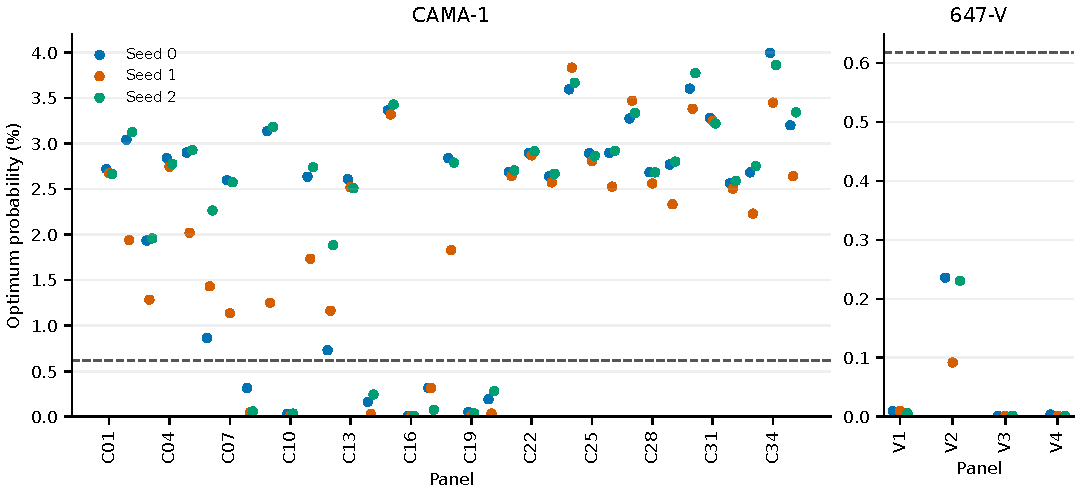
\includegraphics[width=\textwidth]{figures/figureS3.pdf}
\caption{Ideal penalty-QAOA optimum probability for all expanded panels and all three training seeds. The dashed line is uniform feasible sampling, at $100/162$ percent. Panel labels match Table~S11. Left: all CAMA-1 panels. Right: the four 647-V panels selected by measurement coverage.}
\end{figure}

\clearpage
\section{Reproducing the added experiments}
The added code and results are included in the reproducibility package. Run \texttt{prepare\_revision.py} to reproduce the frozen panel design from the supplied source tables. Run \texttt{revision\_experiments.py} with \texttt{--mode classical}, \texttt{--mode panels}, \texttt{--mode grover} and \texttt{--mode rescore} for the four computations. The first three modes produce independent result files. Rescoring uses the saved large-circuit feasible probabilities when available. Run \texttt{python -m unittest test\_revision -v} for numerical and search checks, then \texttt{build\_revision\_outputs.py} to regenerate the supplemental tables and panel figure. Script SHA-256 hashes are listed below; source-table hashes and panel membership are preserved in \texttt{evidence/revision\_design.json}.

\begin{itemize}

\item \texttt{prepare\_revision.py}\newline {\footnotesize\texttt{ad71abd57e05fd902c7a28cf3426c5a1\allowbreak e888fca6d9d23454ef1622b6c0b494e0}}.

\item \texttt{revision\_experiments.py}\newline {\footnotesize\texttt{232a3e45f773b6e3817dcd4a4f88f2f5\allowbreak 9f0940d6595bbc99bc080df60ab0e6f3}}.

\item \texttt{revision\_noiseless.py}\newline {\footnotesize\texttt{a5357753b6e8bbd86e2d941827f7cb2e\allowbreak 605eb321d1e67dd48a85765d1b3f41a7}}.

\item \texttt{test\_revision.py}\newline {\footnotesize\texttt{5acaa95aab14a7f15a9c538dc9ea5235\allowbreak e0b920dd7f33db5e8a69ee381b9eaf0a}}.

\item \texttt{test\_completed\_revision.py}\newline {\footnotesize\texttt{193ea836bd9373b2f38cb808f554f097\allowbreak 4c0286db043e6a7397a916d7438fa5e6}}.

\item \texttt{test\_noiseless\_revision.py}\newline {\footnotesize\texttt{8ddcfee1996c5f492483b8ae645b0ed1\allowbreak cf40e37c9e94c9b48eb3eba19bf1c73f}}.

\item \texttt{build\_revision\_outputs.py}\newline {\footnotesize\texttt{8d0f6d9e196eed0d86d38f312f6c9e11\allowbreak 989ef4d0298dcea4c1077411a029331b}}.

\item \texttt{rewrite\_prose.py}\newline {\footnotesize\texttt{ed6bc7c885976bd151baecb84dd7782e\allowbreak ef3092632a6c34e761aa403643cc7171}}.

\item \texttt{integrate\_revision.py}\newline {\footnotesize\texttt{4b76905a18f377473b76485c935ee015\allowbreak 7f0ba5c21b1203327fa892ecda702be7}}.

\item \texttt{integrate\_noiseless.py}\newline {\footnotesize\texttt{4892851fb7db5534a0a77f223e22614c\allowbreak 5df1838e2fcc793e8caa188394b39c21}}.

\item \texttt{revision.sbatch}\newline {\footnotesize\texttt{cbf13814e1782192d8c690891f6f4f2f\allowbreak d61b6a5ea91576e61b9fa70a26322cd2}}.

\item \texttt{noiseless\_revision.sbatch}\newline {\footnotesize\texttt{ba6ead793b8710fdc832b543ed4e8134\allowbreak 2aad3c61c369eacf3974a1553e6e1b2f}}.

\end{itemize}

\clearpage
\section{Complete task inventory}
The inventory lists all 25 completed tasks by circuit width, nonzero dose choices, UTC date/time in 2026 and UUID, including the six original reference tasks.
\begin{itemize}
\item 6q, $D=2$, 07-03 03:33: \texttt{24d41998-5edf-44bf-93a4-60fca948ae8c}.
\item 6q, $D=2$, 07-03 05:16: \texttt{98cb6dee-1d5d-4aec-9122-6a1c390a2608}.
\item 6q, $D=2$, 07-11 07:10: \texttt{c8ea4f7a-a64e-49d2-a7f8-f1ac1eff2136}.
\item 8q, $D=2$, 07-03 05:25: \texttt{4e307518-f350-4843-98ab-06f91315c190}.
\item 8q, $D=2$, 07-11 07:12: \texttt{e1a915b0-ff23-4769-8289-bfb7fcb0f74b}.
\item 9q, $D=3$, 07-03 05:33: \texttt{e88a4bac-5f06-4b2c-bcc8-69a20d23e527}.
\item 10q, $D=2$, 07-03 05:41: \texttt{9fcd57c3-97a5-4070-929d-d4ba5b7284f9}.
\item 10q, $D=2$, 07-11 07:19: \texttt{fad4ee6f-3815-4d92-af93-dbd2c19ec6a4}.
\item 12q, $D=2$, 07-11 07:25: \texttt{48d52888-7f37-4931-a135-8f831f1a208e}.
\item 12q, $D=3$, 07-03 05:51: \texttt{5cecf3e8-853e-448d-b296-d8bd2ef9f5e0}.
\item 14q, $D=2$, 07-11 07:38: \texttt{1ebf3086-bb62-48fc-9bdb-0df1dedd62cf}.
\item 15q, $D=3$, 07-03 06:03: \texttt{4d659093-99b5-4d58-9063-cd20724f7a98}.
\item 15q, $D=3$, 07-11 07:48: \texttt{566d8e0f-b67b-4786-86fa-3b112aaf15bd}.
\item 18q, $D=3$, 07-11 06:06: \texttt{4b60729f-56e1-45d5-a2d6-fec25d56c84c}.
\item 18q, $D=3$, 07-11 07:55: \texttt{b3fd2bd7-1b51-48e1-9c63-cbe7d55e1120}.
\item 18q, $D=3$, 07-12 13:37: \texttt{014e4aba-2301-4b48-87ba-28c46e97e84f}.
\item 20q, $D=5$, 07-11 08:09: \texttt{abdccbd0-9b84-4ba1-b5a7-91c6e0403be6}.
\item 20q, $D=5$, 07-12 13:47: \texttt{b4079656-2649-4163-9025-133821ff1bdd}.
\item 21q, $D=3$, 07-11 06:09: \texttt{fa0c9bef-c035-4232-a77b-75970696b227}.
\item 21q, $D=3$, 07-11 08:02: \texttt{30a44a65-2124-4664-9720-7d3d53e7498e}.
\item 21q, $D=3$, 07-12 13:40: \texttt{44849fe4-b8c2-4128-8792-ae5ef06009eb}.
\item 25q, $D=5$, 07-11 08:17: \texttt{e69c31e1-b34e-4869-bae9-217de933cb7d}.
\item 25q, $D=5$, 07-12 13:54: \texttt{b1386480-d348-4a01-ae1a-dbecf6d2a934}.
\item 30q, $D=5$, 07-11 08:23: \texttt{bb016dac-cabb-4e80-b568-0c0818917ab6}.
\item 35q, $D=5$, 07-11 08:33: \texttt{cfdf6f35-0141-46b3-a059-7f9e9fc85b9c}.
\end{itemize}


\clearpage
\section{Reproduction}
The reproducibility repository is \url{https://github.com/itsShrizon/warm-start-qaoa-drug-response-reproducibility} (release v1.2.0). Compile \texttt{reproduction/overleaf/supplement.tex} for Tables~S1--S11 and Figures~S1--S3: sampling controls, solution quality, repeated executions, classical search, weight sensitivity, mixer comparisons and expanded panels.

From the package directory, run \texttt{python reanalysis.py} to analyze the bundled records, then \texttt{python build\_figures.py}. Run \texttt{python -m unittest discover -p test\_reanalysis.py -v} for circuit and scorer checks. Analysis runs offline; the package records Python, NumPy, matplotlib and PennyLane versions.

Run \texttt{python quality\_analysis.py} for score distributions and greedy search, and \texttt{python sensitivity.py} for the frozen panel experiment. Every seed is retained; floating-point differences can affect reruns across platforms. Pawsey outputs and execution metadata are archived. Run \texttt{python build\_improvement\_outputs.py} for the added tables and figure, and \texttt{python -m unittest discover -p test\_improvements.py -v} for independent checks.

Run \texttt{python analyze\_recovered\_hardware.py} to check the downloaded tasks and reconstruct their observations, then \texttt{python build\_recovered\_outputs.py} for expanded tables and the repeat plot. Run \texttt{python -m unittest discover -p test\_recovered\_hardware.py -v} to check enumeration through 35 qubits, agreement with the original six records, duplicate handling and grouping by circuit identity.

The directory \texttt{analysis/larger\_noiseless/} contains the submitted package, completed archive, four result JSON files, Slurm logs and accounting record. The archive includes the final batch script and code. Recalculate with \texttt{python larger\_noiseless.py --qubits 18 --output result.json}, substituting 20, 21 or 25. Run \texttt{python build\_larger\_outputs.py} to check saved outputs and generate Tables~S6--S7, then \texttt{python build\_figures.py} for the two-panel feasibility figure. Run all scientific checks with \texttt{python -m unittest discover -p test\_*.py -v}.
\end{document}
